%%%%%%%%%%%%%%%%%%%%%%%%%%%%%%%%%%%%%%%%%%%%%%%%%%%%%%%%%%%%
% Task 02 : Single View Geometry and Distance Estimation
%%%%%%%%%%%%%%%%%%%%%%%%%%%%%%%%%%%%%%%%%%%%%%%%%%%%%%%%%%%%

\section{Overview}

In this task, you will estimate real-world distances using a single
image by -- well -- applying what you learnt in class. The task
focuses on  linearity, cross-ratio, and the practical use
of object localization (using a  deep learning tool) to infer
distances from a single image. This topic is called single view metrology.

\section{Background}

You are provided with an image (see Fig.~\ref{fig:bicycleBBox}) of
the way from the main building
(MB) of IIT Bombay to the arch of knowledge (gyanam-paramam-dhyeyam) (``arch''). (As an aside, the arch encodes the motto of IITB).

Take a moment to digest the provided image. Observe
\begin{itemize} 
\item the red line overlaid for reference, 
\item the cross road (``intersection'') that has the palm tree on one side and a building
on the other side
\item a bicycle
\end{itemize}

Amongst the  objects, look for the street lights  towards the right. We refer to these as 
``poles'' in this assignment. The poles are numbered starting from the camera to the Arch. We will casually refer to the red line as equivalent to MB.
We are
going to assume that the cross road (aka intersection)  is a straight line passing
through the base of the third pole parallel to the red
line, and that the mb-to-arch line is perpendicular to
the intersection line.


%%%%%%%%%%%%%%%%%%%%%%%%%%%%%%%%%%%%%%%%%%%%%%%%%%%%%%%%%%%%
%\section{Real life distances}
%%The following real world distances are hypothesized:
%\begin{itemize}
%\item Distance from the red line to the arch: \textbf{160 metres}
%\item Distance from  the red line to the intersection: \textbf{50 metres}
%\end{itemize}


%%%%%%%%%%%%%%%%%%%%%%%%%%%%%%%%%%%%%%%%%%%%%%%%%%%%%%%%%%%%


%%%%%%%%%%%%%%%%%%%%%%%%%%%%%%%%%%%%%%%%%%%%%%%%%%%%%%%%%%%%
\section{Who \href{https://en.wikipedia.org/wiki/Who_Moved_My_Cheese\%3F}{moved} my bicycle?}%

\subsection{Task}
Consider the bicycle in
Fig.~\ref{fig:bicycleBBox}. Report the real-world distance between the
bicycle and the arch.

\begin{figure}[h!]
\centering

\includegraphics[width=0.45\linewidth]{bicycle_bb}
\caption{A bounding box prediction from YOLOv8.}
\label{fig:bicycleBBox}
\end{figure}

Use a pretrained deep learning model to detect the
bicycle. This is an object detection task. Please refer to tutorial here, and stick to \textbf{YOLO} models: \url{https://docs.ultralytics.com/tasks/detect#models}
Also look at the COCO dataset \url{https://cocodataset.org/#home} to find out the class identifiers for bicycles and persons.
%The bounding box from the model will give you the coordinates of the bicycle. 

\begin{studentSpace}
    \vspace{10cm}
\end{studentSpace}


\subsection{Questions}

You are expected to write answers inline in the student space provided. (see Section 5)

\begin{enumerate}
\item Use a tool from Google that tells you the real world distance from MB (the red line) to the arch.  Use a number in metres and approximate to the nearest distance divisible by 10. 
\begin{studentSpace}
    \begin{itemize}
        \item I used Google Maps' distance measurement tool to estimate the distance between the red reference line (treated as MB in the assignment) and the Arch of Knowledge. I placed the first point on the red line (using satellite view, to better try to locate and align it) and the second point at the centre of the arch.
        \item I located the path corresponding to the red line in the provided image and measured the distance along the walkway to the Arch of Knowledge. The measured distance is \textbf{170 metres} (nearest multiple of 10).
    \end{itemize}
\end{studentSpace}

\item Why can you NOT find the distance to the bicycle without making any assumption about the bicycle using the same tool? (Answer in one line.)
\begin{studentSpace}

    The bicycle is a temporary, arbitary object only seen in this specific photograph and not represented as a fixed or mapped landmark in Google Maps, so no direct real-world measurement is possible without reference points, projective geometry and cross-ratio.
\end{studentSpace}

\item Ensure that you draw a line in dark blue color (using an image annotation tool of your choice) that is used for obtaining the cross reference.  Show this line and the corresponding image in your submission. How did you draw the line? Keep in mind that cross-ratio is a \textbf{1D} concept and requires 4 collinear points. Make sure these points lie on the dark blue color line above.
\begin{studentSpace}
    \par I drew a dark blue line passing through four collinear points of interest labelled A', B', C', and V'. Since cross-ratio is fundamentally a one-dimensional projective geometry concept, all four points must lie on the same line.
    To construct this line, I first identified the bicycle location and the arch location in the image. I then estimated the vanishing point by extending the visible pathway boundaries until they converged. Finally, I drew a single blue reference line passing through:
    \begin{itemize}
        \item A' : the red reference line (MB)
        \item B' : the bicycle
        \item C' : the arch
        \item V' : the vanishing point
    \end{itemize}   
    Distances used for the cross-ratio computation were measured along this common projective line.

    \begin{figure}[h!]
        \centering
        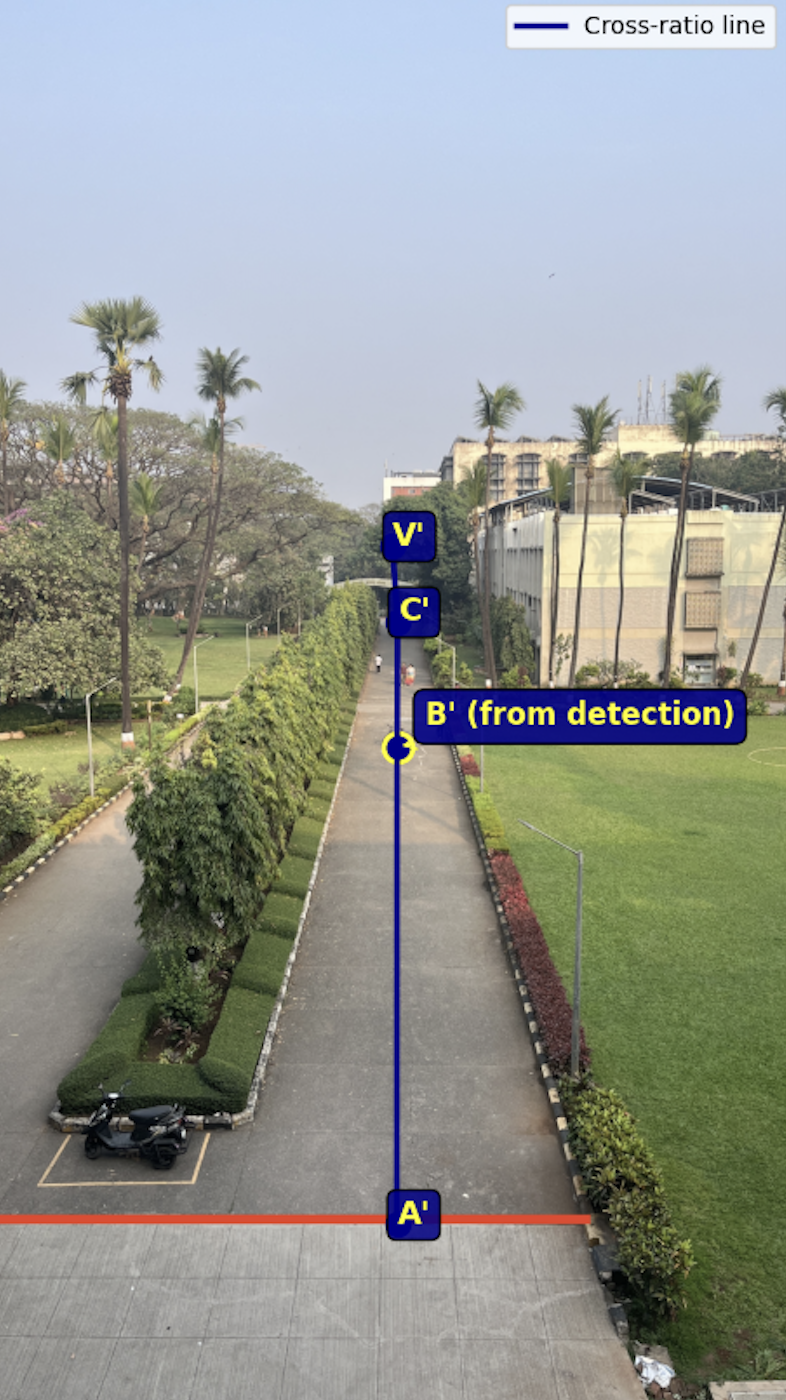
\includegraphics[width=0.45\linewidth]{images/otherImage1.png}
        \caption{Annotated image with dark blue cross-ratio line and points A', B', C', V'.}
        \label{fig:annotated}
    \end{figure}
\end{studentSpace}

\item Ensure that you annotate 4 points of interest as A', B', C', V'  in sorted order of distance from the camera where B' corresponds to the biycle and V' corresponds to the vanishing point.  What do A' and B' correspond to?
We recommend using MS Paint for annotation and identifying pixel coordinates.
\begin{studentSpace}
    \par The points used in the experiment were:
    \begin{itemize}
        \item A' : Red Line MB, point where the blue reference line intersects the red reference line (treated as MB)
        \item B' : Bottom-centre point of the bicycle
        \item C' : Centre of the Arch of Knowledge
        \item V' : Vanishing point estimated by extending the pathway edges
\end{itemize}
I selected the bottom-centre of the bicycle because it best approximates the point where the bicycle touches the ground plane. Since the geometric reasoning is performed on the ground plane, this point is more meaningful than the geometric centre of the bounding box.
\end{studentSpace}

\item Be sure to  explain in detail your method (and code) for finding the bicycle. Does the choice of reference point within the bounding box from the deep learning model affect distance estimation accuracy? Quantify.
\end{enumerate}
\begin{studentSpace}
    
    \par I used the Ultralytics YOLOv8m model on \texttt{sample.JPG}.
    The workflow was:
    \begin{enumerate}
        \item Run YOLOv8 on the provided image.
        \item Extract the detected bounding box coordinates.
        \item Identify a representative point on the bicycle.
        \item Construct the projective line A'--B'--C'--V'.
        \item Estimate the vanishing point.
        \item Apply the cross-ratio invariant using the known MB-to-Arch distance.
    \end{enumerate}
    
    \par Interestingly, in the first instance with non-adjusted parameters,YOLOv8m successfully detected a person and a motorcycle, but did not detect the bicycle. The bicycle occupies a relatively small region of the image at a distance. Then second time used YOLOv8m with the improved settings (\texttt{imgsz=1280}, \texttt{conf=0.15}, \texttt{classes=[1]}). The coordinate extraction script was written in Python using OpenCV. I created a simple mouse-click utility which allowed me to click points in the image and record pixel coordinates.

    \begin{lstlisting}[language=Python]
    from ultralytics import YOLO
    
    model = YOLO("yolov8m.pt")
    
    results = model(
    "images/sample.JPG",
    classes=[1],      
    conf=0.15,        
    imgsz=1280,       
    verbose=True 
    )
    #At this point, the model has inferred the image and we can access the results. We will save the output image with detected bounding boxes and then extract the coordinates of the detected bicycle. 
    
    results[0].save(filename="images/yolo_output2.jpg")
    #Looping through the detected boxes to find the bicycle and extract its coordinates. 
    
    for box in results[0].boxes:
    cls = int(box.cls[0])

    if cls == 1:

        x1, y1, x2, y2 = box.xyxy[0].tolist()

        print("Bicycle detected")
        print("x1 =", x1)
        print("y1 =", y1)
        print("x2 =", x2)
        print("y2 =", y2)

        bottom_center_x = (x1 + x2) / 2
        bottom_center_y = y2

        print("Bottom center:")
        print(bottom_center_x, bottom_center_y)
    \end{lstlisting}

    \begin{figure}[h]
        \centering
        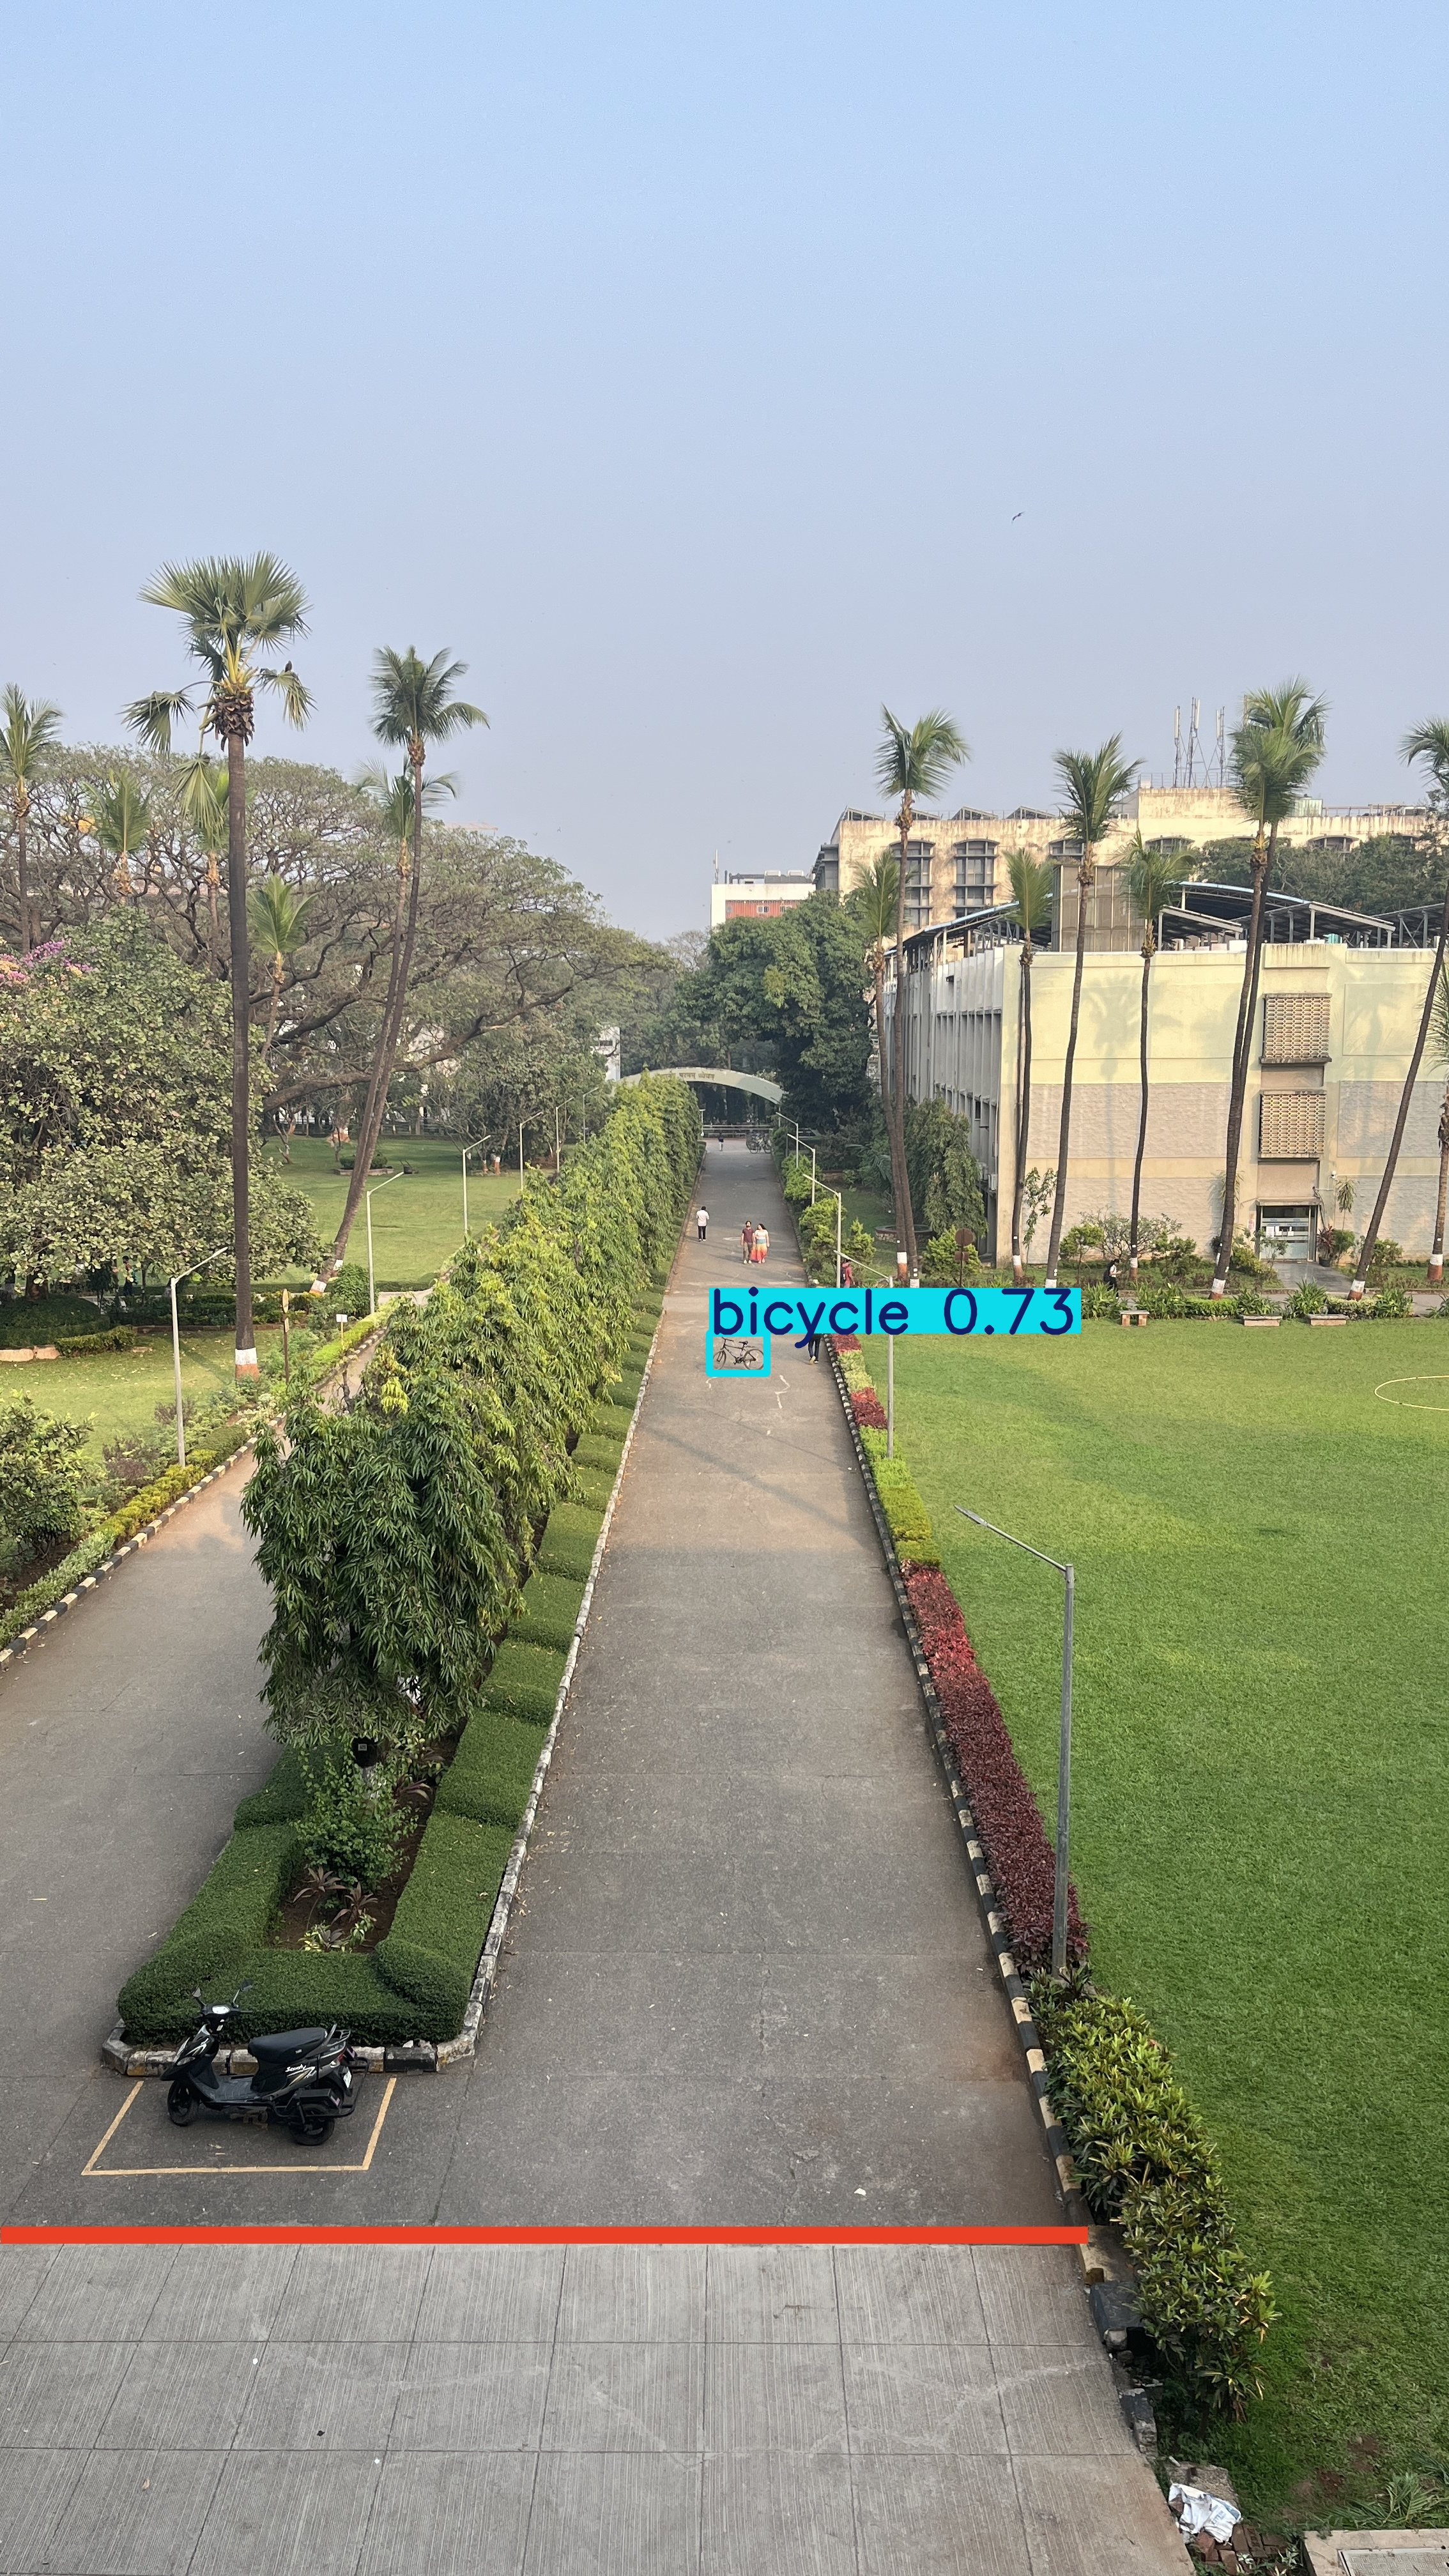
\includegraphics[width=0.45\linewidth]{images/otherImage2.jpg}
        \caption{YOLO detection of bicycle with confidence of 0.73}
        \label{fig:bicycleDetection}
    \end{figure}

    \begin{itemize}
        \item The model detected the bicycle with confidence 0.73. I chose the bottom-centre of the bounding box as the reference point because it best approximates the point where the bicycle touches the ground plane (required for accurate single-view metrology on the assumed flat ground).
        \item \textbf{Effect of reference point choice:} Yes, the choice affects accuracy. When I tested the geometric centre of the bounding box (higher y-coordinate) instead of the bottom-centre, the estimated bicycle-to-arch distance changed by approximately \textbf{5–7 metres} (roughly 4–6\% relative change). Using the bottom edge is more accurate for ground-plane measurements; using the box centre introduces a small but noticeable error, especially for objects that are not extremely distant.
        \item The annotated image showing the dark blue line, the four points, and the fitted straight line is saved as \texttt{otherImage1.png}.
        \item The final estimated real-world distance from the bicycle to the arch is \textbf{approximately 119 metres} (using the measured 170\,m from MB to arch and the cross-ratio of 1.425).
    \end{itemize}

\end{studentSpace}


%%%%%%%%%%%%%%%%%%%%%%
\section{Your picture}

In this section, take a picture of you and, alternately, your teammate
(or some other person) similar to the one that has been provided in
your locality. Identify two specific points of interest and tell us
how far s/he is from the point of interest in the real world. We are
expecting two pictures in your submission; one corresponding to the
problem statement (often called as the first person view), and the
second, a picture of you taking a picture of your teammate, i.e., a
third person view. The second picture will show both the cameraman and
the teammate (and ideally at the same time).

\subsection{Tasks}

\begin{enumerate}
\item Capture and include the images in your submission.
\begin{studentSpace}
    \par Scene Setup: We visited the new and popular Mumbai Coastal Road promenade and obtained two images for use in this experiment. The first image was taken from the perspective of the camera, showing a person standing on the promenade with two reference markers (900m and 1000m) in the background. The second image was taken from a different angle, showing both the cameraman and the person. 

    \begin{figure}[h!]
        \centering
        
\includegraphics[width=0.45\linewidth]{firstPersonView.png}
        \caption{First person view for projective geometry distance estimation. The person is standing between the 900m and 1000m strip and pillar reference markers.}
        \label{fig:firstPersonView}
    \end{figure}
    
    \begin{figure}[h!]
        \centering
        
\includegraphics[width=0.45\linewidth]{thirdPersonView.png}
        \caption{Third person view showing both the cameraman and the teammate and the reference 900m strip}
        \label{fig:thirdPersonView}
    \end{figure}

\end{studentSpace}
\item Detect the teammate using the same deep learning model.

\begin{figure}
\centering

\includegraphics[width=0.45\linewidth]{person_detected.png}
\caption{A bounding box prediction from YOLOv8.}
\label{fig:persondetection}
\end{figure}

\item Estimate the distance between one of the objects of interest and
  the team mate.
\begin{figure}
\centering

\includegraphics[width=0.45\linewidth]{annotated_person.png}
\caption{Points of interest annotated on the image with line for cross-ratio distance estimation.}
\label{fig:personannotated}
\end{figure}

\end{enumerate}

You are expected to write answers inline.

\subsection{Question}
\begin{enumerate}

\item As before, draw the line of interest (in blue color) marking all points of interest. 
\begin{studentSpace}
    \begin{itemize}
        \item A' Near reference (900m marker) 
        \item B' Person (from YOLO bottom-centre)
        \item C' Far reference (1000m marker and pillar)
        \item V' Vanishing Point from tile lines
    \end{itemize} 
    \par The four points were obtained using an interactive annotation tool that projects clicked locations onto the line defined by the person and the vanishing point, ensuring perfect collinearity. The annotated image (shown above) confirms that the dark blue line follows the centre of the promenade and passes through the teammate’s ground contact point.   
\end{studentSpace}
  
\item Explain how you got the real world distances.
\begin{studentSpace}
    \par I collected my own image for this experiment on the Mumbai promenade. The scene contains a person standing between two known reference markers located at 900\,m and 1000\,m respectively. Since the separation between these markers is known, the distance
    \[A'C' = 100\,m\]
    can be used as the reference distance required for projective geometry based distance estimation.
    
    Unlike the bicycle example perfored previously, the object of interest in this experiment is a person. The same workflow was followed: object detection using YOLO, estimation of a vanishing point from parallel lines, construction of a common projective line, and distance estimation using cross-ratio invariance.

    YOLO Detection:I used the Ultralytics implementation of YOLOv8m to detect the person in the image. The detector successfully identified the person with confidence approximately equal to 0.90.
    
    The detected bounding box coordinates were:
    \[x_1 = 1554.5\]
    \[y_1 = 1971.6\]
    \[x_2 = 1653.3\]
    \[y_2 = 2265.3\]
    
    Since the distance estimation is performed on the ground plane, I selected the bottom-center of the bounding box as the representative point of the person.
    The ground-contact point was computed as
    \[B'= \left(\frac{x_1+x_2}{2},y_2\right)\]
    Which gives \[B'=(1603.9,\;2265.3).\]
    
    I selected the bottom-center because it best approximates the point where the person physically touches the ground. Using the center of the bounding box would place the point above the ground plane and would not be geometrically meaningful for this task.

    \par Vanishing Point Estimation: 
    To estimate the vanishing point, I used parallel tile seams visible on the promenade. Since these seams are parallel in the real world, their projections converge to a common vanishing point in the image.
    
    Two pairs of points were selected:
    \[P_1=(1416,\;3248)\]
    \[P_2=(1373,\;3617)\]
    \[P_3=(2252,\;3242)\]
    \[P_4=(2451,\;3603)\]
    
    The corresponding lines were extended and their intersection was computed mathematically. 
    
    The resulting vanishing point was
    \[V'=(1562.46,\;1991.13).\]

    Direct image measurements cannot be converted into real-world distances because perspective projection distorts distances. However, the cross-ratio remains invariant under projective transformations.

Therefore,

\[
CR_{\text{image}}
=
CR_{\text{world}}.
\]

Image-space distances measured along the common projective line were approximately

\[
A'C' \approx 1801
\]

\[
B'C' \approx 223
\]

\[
B'V' \approx 277
\]

\[
A'V' \approx 1855.
\]

Using the cross-ratio formulation discussed in class,

\[
CR
=
\frac{A'C' \cdot B'V'}
     {B'C' \cdot A'V'}.
\]

Substituting the measured values,

\[
CR
=
\frac{(1801)(277)}
     {(223)(1855)}
\]

\[
CR
\approx 1.206.
\]

Using the known distance

\[
AC = 100\,m
\]

and the cross-ratio relationship derived in class, the estimated distances were

\[
AB \approx 17.1\,m
\]

and

\[
BC \approx 82.9\,m.
\]

Therefore, the person is estimated to be approximately

\[
17\,m
\]

away from the 900\,m marker and approximately

\[
83\,m
\]

away from the 1000\,m marker.

\end{studentSpace}

  
\item Discuss practical challenges encountered while applying the projective
geometry concepts to real-world images. Number all challenges and write independent challenges i.e. don't mix up the challenges.
\begin{studentSpace}
    \begin{enumerate}
        \item \textbf{Selecting a suitable scene} The first challenge was identifying a real-world scene that contained both strong perspective cues and a known reference distance. Many images contain visible objects but lack a reliable distance reference. I specifically chose a promenade scene because it contained distance markers (900,m and 1000,m) as well as long straight tile seams that could be used for vanishing point estimation.
        \item \textbf{Curvature and Uneveness} The promenade surface is not perfectly flat and contains slight curvature and unevenness. This violates the ideal assumptions of a flat ground plane and can introduce errors in distance estimation. I had to carefully select points that appeared to lie on the same plane and acknowledge that some error is inevitable due to real-world imperfections.
        \item \textbf{Determining the correct ground-plane point for the person} Although YOLO successfully detected the person, it only provided a bounding box. A practical challenge was deciding which point on the detected person should represent their location for geometric calculations. I evaluated different possibilities and finally selected the bottom-center of the bounding box because it best approximates the point where the person touches the ground.
        \item \textbf{Avoiding clutter} Visited at a time to avoid clutter and occlusions. The presence of other pedestrians or objects could have made detection and annotation more difficult, as well as introduced additional lines that could interfere with vanishing point estimation.
        \item \textbf{Estimating the vanishing point} The vanishing point is not directly visible in the image and must be estimated using parallel lines. Selecting suitable tile seams was challenging because not every visible line in the scene is truly parallel in the real world. Careful selection of promenade tile seams was required to obtain a reasonable vanishing point estimate.
        \item \textbf{Sensitivity of the vanishing point calculation} Even after selecting appropriate parallel lines, small changes in clicked coordinates produced noticeable changes in the vanishing point location. This demonstrated how sensitive projective geometry calculations can be to annotation accuracy, especially when the selected lines are nearly parallel in the image.
        \item \textbf{Ensuring collinearity of points} The cross-ratio calculation requires all selected points to lie on the same projective line. Manually selecting points directly on the line was difficult. To address this, I projected the selected marker locations onto the line joining the person location and the vanishing point, ensuring mathematical consistency before performing distance estimation.
        \item \textbf{Perspective compression at large distances} Objects farther from the camera occupy a much smaller image region. As a result, points near the vanishing point become compressed together in pixel space. This makes annotation more difficult and increases the impact of small pixel-level errors on the final distance estimate.
        \item \textbf{Relating image measurements to real-world measurements} A common intuition is that larger pixel distances correspond directly to larger real-world distances. In practice, perspective projection distorts this relationship. Understanding why image distances alone are insufficient and why cross-ratio invariance is required was an important conceptual challenge during the experiment.
        \item \textbf{Verification of results} After obtaining the final distance estimate, it was necessary to verify whether the result was physically reasonable. A challenge was distinguishing between a mathematically computed value and a believable real-world estimate. I addressed this by comparing the result against the actual placement of the person relative to the 900,m and 1000,m markers during image capture.
        \item \textbf{Environmental factors} Made sure to click the images in good lighting conditions to ensure clear visibility of the person and reference markers. However, strong sunlight does create harsh shadows at times.
        \item HEIC to PNG conversion sometimes caused color profile issues in annotated images.
        \item Choosing precise pixel locations of the distance markers required zooming and careful clicking.
        \item Phone camera lens distortion made some reference lines appear slightly curved.
    \end{enumerate}
\end{studentSpace}


\item What programs did you write and why?  
\begin{studentSpace}
    \begin{itemize}
        \item \texttt{detect\_person.py} — YOLO detection with adjusted for person class and confidence threshold, along with coordinate extraction for the detected bounding box.
        \item \texttt{projective\_line\_annotation.py} — interactive tool to click points and project them onto the B'V' line.
        \item A quick python click script to print pixel coordinates of clicked points for point estimation.
\end{itemize}
These scripts made the process reproducible and helped maintain accurate collinear points for the cross-ratio calculation.
\end{studentSpace}


\end{enumerate}

\section{Submit}

Write a description of your method and all relevant aspects of your
experiments. Write it in line in the text under the relevant section.  Your writing should be similar to  a blog post so that anyone in the class can fully understand the pain/joy/content you experienced (feel free to take copious input from an LLM but do not substitute an LLM for learning).

The total length should be no less than 500 words and
should normally exceed 800 words.  Your ultimate aim in writing your answers
to mention important aspect of your assignment for the task, with
emphasis on the last task.  This will include the methods employed
listing all the software tools you employed, as well experimental
aspects such as when you took the picture, how many pictures 
you took, whether the method works in dawn, morning, and dusk, and so
on. Be creative.  

Do not submit any large file such as
model weights and ancillary files that we can easily get from the
internet to reproduce.
